\chapter{Seminarios}
\section{Seminario 1}
\begin{enumerate}
    \item Sea $A'(x)=a(x)$, probar que para toda función $\phi(x)$ se tiene la equivalencia
    $$\phi'(x)+a(x)\phi(x)= \iff \left(e^{A(x)}\phi(x) \right)'=0 $$
    Como aplicación, resolver la ecuación diferencial $y' + a(x)y = 0$.
    \begin{sol}
    
        \textit{a)} Por la regla de Leibnitz, $$e^{A(x)}(A'(x)\phi(x)+\phi'(x))=0 \: \iff \: a(x)\phi(x)+\phi'(x)=0$$
        
        \textit{b)} $y'+a(x)y=0 \iff (e^{A(x)}y)'=0 \iff e^{A(x)}y=c \iff y=c \cdot e^{-A(x)}$
    \end{sol}
    \item Sea $\gamma(t)=(\cos\: t, \sin \: t)$, calcular el vector velocidad en $t=0$. Idem cuando $$\gamma(t)=(\cos\: t^2, \sin \: t^2)$$
    \begin{sol}
        El vector velocidad es 
        $$\gamma_{*,0}\left(\dfrac{d}{dt}\right)_0=\cancel{-\sin 0} \left( \pd{}{x}\right)_{(1,0)}+\cos0\left( \pd{}{y}\right)_{(1,0)}=\left( \pd{}{y}\right)_{(1,0)}$$     $$\gamma_{*,2\pi}\left(\dfrac{d}{dt}\right)_{2\pi}=\cancel{-\sin 2\pi} \left( \pd{}{x}\right)_{(1,0)}+\cos\pi\left( \pd{}{y}\right)_{(1,0)}=\left( \pd{}{y}\right)_{(1,0)}$$
        Cuando $\gamma(t)=(\cos\: t^2, \sin \: t^2)$:
        $$t=0 \quad \gamma_{*,0}\left(\dfrac{d}{dt}\right)_0=\hfill$$
        $$t=2\pi\hfill$$
        $$t=\sqrt{2\pi} \;  \textcolor{red}{Ejercicio}\hfill$$
        Obsérvese que en el primer caso, el vector velocidad es constante, es decir, la curva (circunferencia) se recorre siempre a la misma velocidad, en cambio, en la segunda, para el mismo obtenemos distintos vectores velocidad.
    \end{sol}
    \item Sea $\phi(x,y)=x^2 \: e^y$, Calcular la aplicación tangente en $(x,y)=(1,3)$.
    \begin{sol}
        Podemos construir los espacios tangentes con las bases
        $$T_p\mathbb R^2=\langle\left(\pd{}{x}\right)_p, \left(\pd{}{y}\right)_p\rangle \quad T_{\phi(p)}\mathbb R= \langle \left(\pd{}{z}\right)_{\phi(p)}\rangle$$
        De forma que la aplicación cotangente es
        $$\begin{array}{rcl}
             T_p\mathbb R^2 & \overset{\gamma_{*,p}}{\longrightarrow} & T_{\phi(p)}\mathbb R  \\
             \left(\pd{}{x}\right)_p & \longmapsto & \gamma_{*,p}\left(\pd{}{x}\right)_p=\lambda\left(\pd{}{z}\right)_{\phi(x)} \\
            \left(\pd{}{y}\right)_p & \longmapsto & \gamma_{*,p}\left(\pd{}{y}\right)_p=\alpha \left(\pd{}{z}\right)_{\phi(x)}
        \end{array}$$
        y donde         $$\lambda=\gamma_{*,p}\left(\pd{}{x}\right)_p \: z=\left(\pd{}{x}\right)_p \gamma^*z=\left(\pd{}{x}\right)_{(1,3)} \: x^2 e^y=(2xe^y)_{(1,3)}=2e^3$$
        \textcolor{red}{TERMINAR $\alpha$}
    \end{sol}
    \item 
    \item 
    \item Dada una matriz cuadrada $C \in M_{n\times n}(\mathbb R)$, definimos la ``curva de matrices'' $\gamma : \mathbb R \longrightarrow M_{n\times n}(\mathbb R)$  por ser $\gamma(t) := e^{tC}$. Calcular la aplicación tangente en $t = 5$. (Se considera a $M_{n\times n}(\mathbb R)$ identificado con $\mathbb R^{n^2}$ tomando como coordenadas de una matriz la colección de sus coeficientes: $x_{ij} (X) :=$ coeficiente $ij$ de la matriz $X$).
    \begin{sol}
        Para calcular la aplicación tangente, basta calcular $\gamma_{*,5}\left( \frac{d}{dt}\right)_5$ y, denominando a los coeficiente de $e^{tC}=\big(b_{ij}\big)$, es decir, $x_{ij}(\gamma(t))=x_{ij}(e^{tC})$, tenemos que $\gamma(t)=(b_{11}, b_{12}, \ldots, \: b_{21}, \ldots, b_{nn})$ (por el isomorfismo expuesto en el enunciado). Ahora bien, entonces
        $$\gamma_{*,5}\left( \frac{d}{dt}\right)_5=\left( \dfrac{d\gamma_{11}}{dt}\right)_5 \left(\pd{}{x_{11}} \right)_{e^{5C}} + \: \cdots \: + \left( \dfrac{d \gamma_{nn}}{dt}\right)_5 \left(\pd{}{x_{nn}} \right)_{e^{5C}}=$$
        $$=\left( x_{11}(C e^{tC})\right)_5 \left(\pd{}{x_{11}} \right)_{e^{5C}} + \: \cdots \: + \left(  x_{nn}(C e^{tC})\right)_5 \left(\pd{}{x_{nn}} \right)_{e^{5C}}=$$
        $$=\left( x_{11}(C e^{5C})\right) \left(\pd{}{x_{11}} \right)_{e^{5C}} + \: \cdots \: + \left(  x_{nn}(C e^{5C})\right) \left(\pd{}{x_{nn}} \right)_{e^{5C}}=C e^{5C}$$
        
    \end{sol}
    \item  Dada una matriz cuadrada $C \in M_{n\times n}(\mathbb R)$, definimos la aplicación $\alpha: M_{n\times n}(\mathbb R) \longrightarrow M_{n\times n}(\mathbb R)$ por la regla $\alpha(X) := CX$, para cada $X \in M_{n\times n}(\mathbb R)$. Calcular la aplicación tangente en $X = A$, para una cierta matriz $A \in M_{n\times n}(\mathbb R)$.  
    \begin{sol} Tomando los coeficientes de las matrices, dado $\alpha(X)=C \cdot X$, $\alpha_{kl}(x)= c_{ij}(x) $
        $$\gamma_{*,A} \left( \pd{}{x_{ij}} \right)_A=\sum_{k=1}^n\sum_{l=1}^n  \left( \pd{\alpha_{kl}}{x_{ij}} \right)_A  \left( \pd{}{y_{kl}} \right)_{CA}=\sum_{k=1}^n\sum_{l=1}^n \delta_{lj} \cdot c_{ki}  \left( \pd{}{y_{kl}} \right)_{CA}=\sum_{k=1}^n  \left( \pd{}{y_{kj}} \right)_{CA}$$
    \end{sol}
\end{enumerate}
\section{Seminario 2}
\begin{ejer}
    \textbf{1.b)} Resolver las ecuaciones diferenciales lineales $(1-x^2)y' + xy = ax,  \quad a \in \mathbb R$
\end{ejer}\begin{sol}
    Para obtener la ecuación como lineal, dividimos por $1-x^2$:
    $$y'+\dfrac{x}{1-x^2} \: y=\dfrac{ax}{1-x^2}$$
    Y resolvemos la ecuación homogénea
    $$y'+\dfrac{x}{1-x^2} \: y=0$$
    
    \underline{Homogénea}
    $$y=k \cdot e^{-\mathlarger{\int} \frac{x}{1-x^2} dx}\overset{1.}{=}k \cdot e^{\frac{1}{2} \: \log\left|1-x^2\right|}=k \cdot \sqrt{\pm (1-x^2)}$$
    $$^{1.} \int \dfrac{x}{1-x^2} \: dx=-\dfrac{1}{2} \int \dfrac{-2x}{1-x^2} \: dx=-\dfrac{1}{2}\log|1-x^2| \qquad \qquad \qquad \qquad \qquad \qquad \qquad \qquad$$
    
    \underline{Particular}
    $$y_p=k(x)\cdot\sqrt{1-x^2} \text{ con } k'(x)=\dfrac{\frac{ax}{1-x^2}}{\sqrt{1-x^2}}=\dfrac{ax}{\left(1-x^2\right)^{\nicefrac{3}{2}}} \: \Rightarrow \: k(x)=\int \dfrac{ax}{\left(1-x^2\right)^{\nicefrac{3}{2}}} \: dx= \dfrac{a}{\sqrt{1-x^2}}$$
    Por tanto, $$y_p=\dfrac{a}{\cancel{\sqrt{1-x^2}}} \: \cancel{\sqrt{1-x^2}}=a$$

    \underline{General}
$$y=a+k \cdot \sqrt{1-x^2} \quad a,k \in \mathbb R$$
    
\end{sol}
\begin{ejer}
    \textbf{2.} Calcular la solución al problema de Cauchy
    $$\left\{ \begin{array}{l}
         y' + y \cos(x) = \sen(x) \cos(x)  \\
         y(0)=1
    \end{array}\right.$$
\end{ejer}
\begin{sol}

    \underline{Homogénea}
    $$y' + y \cos(x) = 0 \: \Rightarrow \: y=k \cdot e^{-\int \cos(x) dx}=k \cdot e^{-\sin(x)}$$

    \underline{Particular}
    $$y_p=k(x) \cdot e^{-\sin(x)} \text{ con } k'(x)=\dfrac{\sin(x) \: \cos(x)}{e^{-\sin(x)}} $$
    $$\: \Rightarrow \: k(x)=\int \dfrac{\sin(x) \: \cos(x)}{e^{-\sin(x)}}dx = e^{\sin(x)}(\sin(x)-1)$$
    $$y_p=\sin x -1$$

    \underline{General}
    $$y=k e^{-\sin(x)}  +\sin(x)-1$$

    \underline{$y(0)=1$}
    $$1=y(0)=\cancelto{1}{e^{-\sin(0)}} k + \cancelto{0}{\sin(0)}-1=k-1=1 \: \Rightarrow \: k=2 \: \Rightarrow \: y=2e^{-\sin(x)} \sin(x)-1$$
    
\end{sol}
\begin{ejer} \textbf{4.a)}
    Resolver las siguientes ecuaciones diferenciales, lineales si se considera a $x$ como función de $y$:
    $$y'=\dfrac{1}{x\cos y+\sin 2y}$$
    que no es lineal. En cambio, invirtiendo la dependencia
    $$\dfrac{dy}{dx}=\dfrac{1}{x\cos y+\sin 2y} \iff \dfrac{dx}{dy}=x \cos y+\sin 2y \iff \dfrac{dx}{dy}-\underbrace{\cos y}_{a(y)} \cdot \: x=\underbrace{\sin 2y}_{b(y)}$$
    obtenemos un ecuación diferencial lineal.
\end{ejer}
\begin{sol}
    Dada la similitud con el ejercicio anterior, procedemos con la \underline{solución particular} directamente (cambiando el signo eh):
    $$x_p=k(y) \cdot e^{\sin(y)} \text{ con } k'(y)=\dfrac{\sin 2y}{e^{\sin(y)}} $$
    $$\: \Rightarrow \: k(y)=\int \dfrac{\sin 2y}{e^{\sin(y)}} \: dy= \int \dfrac{2 \sin (y) \cos (y)}{e^{\sin(y)}} \: dy= -2 e^{\sin(y)}{(\sin(y) + 1)} $$
    $$k=-2e^{-\sin(x)}(\sin(x)+1) \: \Rightarrow \: y_p=-2(\sin(x)+1)$$

    \underline{General}
    $$x=ke^{\sin(y)}-2 (\sin(y) + 1)$$
\end{sol}

\section{Seminario 3}
\begin{ejer}
    \textbf{5.b)} Resolver la siguiente ecuación diferencial de variables separadas: 
    $$3e^x \tg(y)dx + (2 - e^x) \sec^2(y)dy = 0$$
\end{ejer}
\begin{sol}
    Se trata de una ecuación diferencial de variables separadas, por lo que vamos a separarlas:
    $$3e^x \tg(y)dx + (2 - e^x) \sec^2(y)dy = 0 \: \iff \: 3e^x \tan(y)dx = (e^x - 2) \sec^2(y)dy \: \iff $$
    $$\: \iff \: \frac{3e^x}{e^x - 2} dx = \dfrac{\sec^2(y)}{\tan(y)}dy \: \iff \: \frac{3e^x}{e^x - 2} dx = \dfrac{1+\tan^2(y)}{\tan(y)}dy \: \iff \: \frac{3e^x}{e^x - 2} dx - \left(\dfrac{1}{\tan(y)}+\tan(y)\right) dy=0$$
    Integrando la expresión en $x$, con el cambio de variable $t:=e^x-2$ ($dt=e^x dx$)
    $$3\int \dfrac{e^x}{e^x-2}dx= 3 \int \dfrac{dt}{t}=3 \log|t|=3\log|e^x-2|$$
    y la segunda
    $$\int \dfrac{1}{\tan(y)}\: dy+\int \tan(y)\:  dy=\log|\sin(y)|-\log|\cos(y)|=\log\left|\dfrac{\sin(y)}{\cos(y)}\right|=\log|\tan(y)|$$
    por tanto,
    $$d\left(3\log|e^x-2|)-\log|\tan(y)|\right)=d\left(\log\left|\dfrac{(e^x-2)^3}{\tan(y)}\right|\right)=0 \: \iff \: \log\left|\dfrac{(e^x-2)^3}{\tan(y)}\right|=c \: \iff \: $$
    $$\iff \: \dfrac{(e^x-2)^3}{\tan(y)}=e^c=k \: \iff  \: \dfrac{(e^x-2)^3}{k}=\tan(y)$$
    y por tanto la solución es 
    $$\boxed{y=\arctan\left(\dfrac{(e^x-2)^3}{k}\right)} \qquad k \in \mathbb R$$
\end{sol}
\begin{ejer}
    \textbf{8.b)} Comprobar que las siguientes ecuaciones diferenciales son exactas y resolverlas:
    $$(\overbrace{\sin(xy) + xy \cos(xy)}^{A})dx + \overbrace{(x^2 \cos(xy))}^Bdy = 0$$
\end{ejer} 
\begin{sol} Comprobemos la exactitud
    $$\pd{A}{y}= x \cos(xy) + x \cos(xy) - x^2y \: \sin(xy)=2x \: \cos(xy)+x^2y\: \sin(xy)$$
    $$\pd{B}{x}=2x \: \cos(xy)-x^2y\: \sin(xy)$$
    verificándose el criterio de exactitud, por tanto, resolvemos como 1-forma exacta. Calculando un potencial $F(x,y)$ tal que $\omega =dF$, es decir,
    $$\left\{ \begin{array}{l}
         \pd{F}{x}=A=\sin(xy) + xy \cos(xy) \\
         \pd{F}{y}=B=x^2 \cos(xy) \: \Rightarrow \: F(x,y)=x^2\: \dfrac{\sin(xy)}{x}+\varphi(x)=x \:  \sin(xy)+\varphi(x)
    \end{array}\right.$$
    Sustituyendo en $A$, 
    $$\pd{}{x} \: (x \:  \sin(xy)+\varphi(x))=A \: \iff \: \sin(xy)+xy\cos(xy)+\varphi'(x)=\sin(xy) + xy \cos(xy) \: \iff $$ $$ \: \iff \: \varphi'(x)=0 \: \iff \: \varphi(x)=c$$
    Por lo que $F(x,y)=x \:  \sin(xy)+c$ y por tanto la solución a la ecuación diferencial es $F(x,y)=c'$, es decir, 
    $$x \:  \sin(xy)=k \: \Rightarrow \: \boxed{y=\dfrac{\arcsin({\nicefrac{k}{x}})}{x}} \quad c'-c=:k \in \mathbb R$$
\end{sol}
\begin{ejer}
    \textbf{9.b)} Resolver la ecuación diferencial homogénea:
    $$y'=\dfrac{y-x}{y+x}$$
\end{ejer}
\begin{sol}
    $$y'=\dfrac{y-x}{y+x} \: \iff \:  y'=\dfrac{\frac{y}{x}-1}{\frac{y}{x}+1}=\dfrac{u-1}{u+1}=(xu)'=u+xu' \: \Rightarrow \: xu'=\dfrac{u-1}{u+1}-u$$
    $$\: \Rightarrow \: x \: \dfrac{du}{dx}=\dfrac{u-1}{u+1}-u =\dfrac{u-1-u(u+1)}{u+1}=\dfrac{u^2-1}{u+1}=\dfrac{(u-1)\cancel{(u+1)}}{\cancel{u+1}}=u-1$$
    Es decir, 
    $$\dfrac{du}{u-1}-\dfrac{dx}{x}=0 \: \iff \: d \left( \log\left|\dfrac{u-1}{x}\right|\right)=0\: \iff \: \log\left|\dfrac{u-1}{x}\right|=c \: \iff \: u-1=x \cdot e^c $$
    y deshaciendo el cambio de variable,
    $$\dfrac{y}{x}-1=x \cdot e^c \: \iff \: y=x(x \cdot e^c+1)$$
    Es decir,
    $$\boxed{y=k\cdot x^2+x=x(k\cdot x+1)} \quad k \in \mathbb R^+$$
\end{sol}
\begin{ejer}
    \textbf{11.d)} Resolver la ecuación de Bernoulli:
    $$3xy'-2y=\dfrac{x^3}{y^2}$$
\end{ejer}
\begin{sol}
    Reordenándola,
    $$3xy'=2y+\dfrac{x^3}{y^2} \: \iff \: y'=\dfrac{2y}{3x}+\dfrac{x^3}{3xy^2} \: \iff \: y'=\dfrac{2y}{3x}+\dfrac{x^2}{3y^2}=\dfrac{2}{3x}\: y + \dfrac{x^2}{3} \: y^{-2}$$
    y dividiendo por $y^{-2}$ (multiplicando por $y^2$),
    $$y^2 \: y'=\dfrac{2}{3x} \: y^3 + \dfrac{x^2}{3} \: \underset{z'=3y^2y'}{\overset{z=y^3}{\iff}} \: z'=\cancel{3}\dfrac{2}{\cancel{3}x} z + \cancel{3}\dfrac{x^2}{\cancel{3}} \: \Rightarrow \: z'-\dfrac{2}{x}z=x^2$$

    \underline{Homogénea}
    $$z'-\dfrac{2}{x}z=0 \: \iff \: z=k\cdot e^{-\int \nicefrac{2}{x} \: dx}=k \cdot e^{\log|x^2|}=k \cdot x^2$$

    \underline{Particular}
    $$z_p=k(x)\cdot x^2 \text{ con } k'(x)=\dfrac{x^2}{x^2}=1 \: \Rightarrow \: k(x)=x \: \Rightarrow \: z_p=x^3$$

    \underline{General}
    $$\boxed{z=x^3+k \cdot x^2}$$

    Deshaciendo pues el cambio de variable $z=y^3$, 
    $$y^3=x^2(x+k) \: \iff \: \boxed{y=\sqrt[3]{x^2(x+k)}} \quad k \in \mathbb R$$
\end{sol}

\begin{ejer}
    \textbf{13.d)} Resolver
    $$(x-2y-1)dx+(3x-6y+2)dy=0$$
\end{ejer}
\begin{sol}
    Reordenando, 
    $$\dfrac{-x+2y+1}{3x-6y+2}=\dfrac{dy}{dx}=y'$$
    que es una ecuación del tipo cociente de rectas. Dado que $3x-6y$ es $-3(-x+2y)$, las rectas son paralelas. Llamamos ahora $z:=-x+2y+1$, 
    $$\dfrac{-x+2y+1}{3x-6y+2}=\dfrac{z}{-3z+5}$$
    y derivando $z$, 
    $$z'=-1+2y'=-1+2\:\dfrac{z}{-3z+5}=\dfrac{3z-5+2z}{-3z+5}=\dfrac{5z-5}{-3z+5}$$
    por lo que 
    $$\dfrac{dz}{dx}=\dfrac{5z-5}{-3z+5} \: \iff \: \dfrac{-3z+5}{5z-5}dz - dx=0$$
    La primera integral es
    $$\int \dfrac{-3z+5}{5z-5}dz =\int \dfrac{-3z}{5z-5}+\dfrac{1}{z-1} \: dz=-\dfrac{3}{5}\int\dfrac{z}{z-1}dz+\int\dfrac{1}{z-1}dz=$$
    $$=-\dfrac{3}{5}\int\left(\dfrac{1}{z-1}+1\right)dz+\int\dfrac{1}{z-1}dz=-\dfrac{3}{5}(z+\log|z-1|)+\log|z-1|=-\dfrac{3z}{5}+\dfrac{2}{5}\log|z-1|$$
    Recapitulando,
    $$\dfrac{-3z+5}{5z-5}dz - dx=0 \: \iff \: d \left( -\dfrac{3z}{5}+\dfrac{2}{5}\log|z-1| - x \right)=0 \: \iff \: -\dfrac{3z}{5}+\dfrac{2}{5}\log|z-1| - x =c$$
    y deshaciendo el cambio de variable $z:=-x+2y+1$,
    $$-\dfrac{3(-x+2y+1)}{5}+\dfrac{2}{5}\log|-x+2y+1-1| - x =c \: \iff \: \boxed{\dfrac{2}{5} \log|x - 2 y| - 8 x + 6 y + 3 = c \: } \; \; \; \;  c \in \mathbb R$$
\end{sol}
\begin{ejer}
    \textbf{14.b)} Cada una de las siguientes ecuaciones diferenciales admite como factor integrante una función que depende solo de una de las variables. Búsquese dicho factor y resuélvase la ecuación:
    $$(x+\sin(x)+\sin(y))dx+\cos(y)dy=0$$
\end{ejer}

\section{Seminario 4}
\begin{ejer}
    \textbf{15.a)}  Resolver la siguiente ecuación diferencial sabiendo que admite como factor integrante una función del tipo que se indica:
    $$\underbrace{(3x+2y+y^2)}_A dx+\underbrace{(x+4xy+5y^2)}_B dy=0; \; \mu = \varphi(x+y)$$
\end{ejer}
\begin{sol}
    Hallemos $\mu$ tal que 
    $$\pd{\mu A}{y}=\pd{\mu B}{x}$$
    Por un lado
    $$\pd{(3x\mu+2y\mu+\mu y^2)}{y}=$$
    \textcolor{red}{TERMINAR}
\end{sol}
\begin{ejer}
    \textbf{16.} Resolver:
    
    a) $2xy'(x^2+y^2)=y(y^2+2x^2)$
    \begin{sol}
        Véase que es una ecuación homogénea, ya que 
        $$y'=\dfrac{y^3+2x^2y}{2x^3+2xy^2}$$
        entonces, dividiendo todo por $x$,
        $$y'=\dfrac{\nicefrac{y^3}{x}+2xy}{2x^2+2y^2} \; \overset{u=\nicefrac{y}{x}}{\Rightarrow} \; y'=(xu)'=u+xu'=\dfrac{\nicefrac{x^3u^3}{x}+2x^2u}{2x^2+2x^2u^2}=\dfrac{u^3x^2+2x^2u}{2x^2+2x^2u^2}=\dfrac{\cancel{x^2}(u^3+2u)}{\cancel{x^2}(2+2u^2)} \; \iff \;$$
        $$\iff \; u'=\dfrac{u^3\cancel{+2u}\cancel{-2u}-2u^3}{x(2+2u^2)}=\dfrac{-u^3}{x(2+2u^2)} \; \iff \; \dfrac{2+2u^2}{u^3} du + \dfrac{dx}{x}=0 \; \iff \;$$
        donde integrando el primer miembro
        $$2\int \dfrac{1}{u^3} + \dfrac{u^2}{u^3} \: du = 2 \int \dfrac{du}{u^3} + \int \dfrac{1}{u} \: du=2\left(\dfrac{-1}{3} u^{-2}\right)+2\log|u|=\dfrac{-2}{3u^2} +\log|u^2|$$
        Luego, recapitulando, 
        $$d\left(\dfrac{-2}{3u^2} +\log|u^2|+ \log|x| \right)=0 \; \iff \; \dfrac{-2}{3u^2} +\log|u^2|+ \log|x|=c $$
        así pues, deshaciendo el cambio de variable $u=\nicefrac{y}{x}$, 
        $$\dfrac{-2x^2}{3y^2} +\log\left|\nicefrac{y^2}{x^2}\right|+ \log|x|=c \; \iff \; \boxed{\log\left|\frac{y^2}{x}\right|=c+\dfrac{2x^2}{3y^2}} $$
    \end{sol}

    c) $x^2y'+2x^3y=y^2(1+2x^2)$

    e) $(x^4 \log (x)-2xy^3)dx+3x^2y^2dy=0$
    
\end{ejer}
\begin{ejer} \textbf{3.}
    Hallar la familia de curvas para las cuales la longitud del segmento que determina la tangente en el eje de las ordenadas es igual a la abcisa del punto de tangencia.
\end{ejer}
\begin{sol}
    Considerando el punto de tangencia $p_o=(x_o,y_o)$, la recta tangente es $$y-y_o=y'(x-x_o)$$
    El corte con el eje de las ordenadas (eje $OY$) viene se halla haciendo $x=0$, por tanto, $y=y_o-x_oy'$ y el corte de la tangente con el eje $OY$ es en el punto $p_2=(0,y_o-x_oy')$. 

    De esta forma, queremos esta distancia con la abscisa de $(x_o,y_o)$, esto es, $(x_o,0)$:
    $$y_o-x_oy' = x_o \; \iff \; y'=-\dfrac{x_o+y_o}{x_o}=-1-\dfrac{y_o}{x_o}$$
   y como se debe verificar para cualquier punto de tangencia, 
   $$\dfrac{dy}{dx}=-1-\dfrac{y}{x}\; \iff \;y'=(xu)'=u+xu'=-1-u\; \iff \; u'=-\dfrac{1+2u}{x} \; \iff \; $$
    $$\; \iff \; \dfrac{du}{1+2u}+\dfrac{dx}{x}=0 \; \iff \; d \left( \log|2u+1| + \log |x|  \right)=0 \; \iff \; \log \left| \dfrac{2u+1}{x} \right|=c \; \iff $$
    $$\iff \; \dfrac{2\nicefrac{y}{x}+1}{x}=k \; \iff \; y=\dfrac{kx^2}{2}-\dfrac{x}{2} \; \iff \; \boxed{y=\dfrac{1}{2}x(kx-1)}$$
\end{sol}
\begin{ejer} \textbf{7.}
    Un punto material de masa igual a 1 gramo se mueve en línea recta debido a la acción de una fuerza que es directamente proporcional al tiempo, calculado desde el instante $t = 0$, e inversamente proporcional a la velocidad del punto. A los diez segundos la velocidad es igual a $50$ cm/s y la fuerza igual a 4 dinas. ¿Qué velocidad tendré el punto al cabo de un minuto del comienzo del movimiento?
\end{ejer}
\begin{sol}
Sea $F$ la fuerza, es proporcional al tiempo $t$, e inversamente proporcional a la velocidad $x'$, entonces 
$$F(t)=\alpha \; \dfrac{t}{v}$$
y dadas las condiciones inciales $v(10)=0,5$m/s $F(10)=4$ dinas = $4 \cdot 10^{-5}N$, podemos hallar la constante 
$$\alpha=\dfrac{F(10) \cdot v(10)}{10}=\dfrac{50 \cdot 4}{10}=20 \; \Rightarrow \; F=20 \; \dfrac{t}{v}$$
y ahora, dado que $F=m \cdot v'$, con $m=1$g, 
$$F=m \cdot v'=1 \cdot v'=20\: \dfrac{t}{v} \; \iff \; v'=20 \: \dfrac{t}{v} \; \iff \; \dfrac{dv}{dt}=20 \: \dfrac{t}{v} \; \iff \; v\: dv -20 t \: dt=0 \; \iff$$
$$ \iff \; \dfrac{v^2}{2}-10 t^2=c$$
Así que, dadas las condiciones inciales, 
$$v(t)=\sqrt{2(c+10t^2)} \; \Rightarrow \; v(10)=50=\sqrt{2(c+10 \cdot 10^2)} \; \Rightarrow \; c =250 $$
de forma que la expresión general de la velocidad es 
$$v(t)=\sqrt{500+20t^2} \; \Rightarrow \; v(60)=\sqrt{72.500}$$
\end{sol}
\begin{ejer}
    \textbf{18.b)} Calcular las trayectorias ortogonales a cada una de las siguientes familias de curvas:
    \begin{itemize} \vspace{-3mm}
        \item[a)] Las circunferencias $x^2 + y^2= c, \: c \geq 0$.
        \item[b)] Las circunferencias $x^2 + y^2= 2cx$.
        \begin{sol}
            Las trayectorias tangentes, derivando implícitamente, satisfacen la ecuación:
            $$2x+2yy'=2c \: \iff \; y'=\dfrac{c-x}{y} \quad (y \neq 0)$$
            Teniendo en cuenta que la recta perpedicular a una dada (sea su pendiente $\alpha$) es $-\frac{1}{\alpha}$, la ecuación de las trayectorias ortogonales es
            $$y'=\dfrac{y}{x-c} \; \iff \; \dfrac{1}{y}dy-\dfrac{1}{x-c}dx=0 \; \iff \; d\left(\log|y|-\log|x-c| \right)=0 \; \iff \; \log\left|\dfrac{y}{x-c}\right| =k$$
            así pues, la solución es 
            $$y=k(x-c) \qquad k \in \mathbb R^+$$
            Pero esto lo verifica para una sola circunferencia $x^2 + y^2= 2cx$ con $c$ fijo. Despejando $c$, 
            $$c=\dfrac{x^2+y^2}{2x} \; \Rightarrow \; \boxed{y=k\left(\dfrac{x^2-y^2}{2x}\right)}$$
            obtenemos la solución general.
        \end{sol}
        \item[c)] Las parábolas $y = cx^2$.
    \end{itemize}
\end{ejer}
\begin{ejer}
    \textbf{21.} Hallar la familia de curvas que tienen la propiedad de que el segmento de la tangente a cada una de ellas comprendido entre los ejes de coordenadas se divide por la mitad en el punto de contacto.
\end{ejer}
\begin{sol} \textcolor{red}{CREO QUE ESTÁ MAL}
    Sea $(x_o,y_o)$ el punto de tangencia, los cortes con los ejes $(a,0)$ y $(0,b)$, entonces lo que deben cumplir todos los puntos de la curva es que 
    $$d((x_o,y_o),(a,0))=d((x_o,y_o),(0,b)) \; \iff \; \sqrt{(x_o-a)^2+y_o^2}=\sqrt{x_o^2+(y_o-b)^2}$$
    la recta tangente a $y(x)$ en $(0,b)$ tiene por ecuación 
    $$y=b+y'(x_o)x$$
    se debe cumplir que pase por $(a,0)$ y $(x_o,y_o)$, es decir, 
    $$\left\{\begin{array}{ll}
         y_o=b+y'x_o \; & \Rightarrow  \; b=y_o-y'x_o   \\
         0=b+y'a \; & \Rightarrow  \; a=-\dfrac{b}{y'}=x_o-\dfrac{y_o}{y'} 
    \end{array} \right.$$
    La ecuación resultante es pues
    $$\sqrt{\left(\dfrac{y_o}{y'}\right)^2+y_o^2}=\sqrt{x_o^2+(y'x_o)^2}$$
    y como se debe verificar $\forall \: (x_o,y_o)$;
    $$\dfrac{y^2}{(y')^2}+y^2=x^2+(y')^2 x^2 \; \iff \; y^2+y^2(y')^2=(y')^2x^2+(y')^4x^2 \; \iff \; (y')^4 + \left(1-\dfrac{y^2}{x^2} \right)(y')^2-\dfrac{y^2}{x^2}=0 $$
    sea $u:=\nicefrac{y^2}{x^2}$ luego, como ecuación bicuadrada
    $$(y')^2=\dfrac{-(1-u)\pm\sqrt{(1-u)^2+4u}}{2}=\dfrac{-(1-u)\pm(1+u)}{2}$$
    Así, eligiendo el signo,
    \begin{enumerate}
        \item $(y')^2=\dfrac{-(1-u)+(1+u)}{2}=\dfrac{2u}{2}=u \: \Rightarrow \: (y')^2=u=\dfrac{y^2}{x^2} \; \Rightarrow \; y'=\pm \dfrac{y}{x} \; \iff \;$
        
        1.1.$$\dfrac{1}{y}dy-\dfrac{1}{x}dx=0 \; \iff \; \log|y|-\log|x|=c \; \iff \; \boxed{y=kx}$$

        1.2.$$\dfrac{1}{y}dy+\dfrac{1}{x}dx=0 \; \iff \; \log|y|+\log|x|=c \; \iff \; \boxed{y=\dfrac{k}{x}}$$
        
        \item $(y')^2=\dfrac{-(1-u)-(1+u)}{2}=\dfrac{-1+u-1-u}{2}=-1$
    \end{enumerate}
\end{sol}
\begin{ejer}
    \textbf{22.} Demostrar que las curvas cuyas normales pasan por un punto constante son circunferencias.
\end{ejer}
\begin{sol}
    Sea $(x_o,y_o)$ el punto por el que pasan las rectas, estas rectas tienen como ecuación $y-y_o=y'(x-x_o)$, luego sus normales verifican la ecuación:
    $$y-y_o=-\dfrac{1}{y'}(x-x_o) \; \Rightarrow \; y'=-\dfrac{x-x_o}{y-y_o} \; \iff \; (y-y_o)dy+(x-x_o)dx=0 \; \iff $$
    $$\; \iff \; \dfrac{y^2}{2}-y_o y + \dfrac{x^2}{2}-x_o x= c \; \iff \; y^2-2y_oy + x^2-2x_ox=2c=c' \; \iff $$ 
    $$ \iff \: (y^2-2y_oy +y_o^2) + (x^2-2x_ox+x_o^2) =c''=c'+x_o^2+y_o^2  $$
    luego la solución es
    $$\boxed{(y-y_o)^2+(x-x_o)^2=c''} \quad c'' \in \mathbb R^+$$
\end{sol}
\begin{ejer}
    \textbf{24.} Según la ley de Newton, la velociodad de enfriamiento de un cuerpo en el aire es proporcional a la diferencia entre la temperatura T del cuerpo y la temperatura del aire. Si la temperatura del aire es de 20ºC y el cuerpo pasa en 20 minutos
desde 100ºC hasta 60ºC, ¿cuánto tiempo tardará su temperatura en descender
hasta 30ºC?
\end{ejer}
\begin{sol}
    Sea $T$ la temperatura del cuerpo, el enunciado nos dice que $T'=\alpha(T-k_o)$ con $k_o=20$ºC la temperatura del aire. Ahora bien $T(0)=100$ y $T(20)=60$. Así pues, tenemos la ecuación diferencial
    $$T'=\alpha T-20\alpha $$
    que resolveremos como lineal

    \underline{Homogénea}
    $$T'-\alpha T=0 \; \Rightarrow \; T=k \cdot e^{\alpha x}$$

    \underline{Particular}
    $$T_p=k(x) \cdot e^{\alpha x} \text{ con } k'(x)\cdot e^{\alpha x}=-20\alpha \; \Rightarrow \; k(x)=\int \dfrac{-20\alpha }{e^{\alpha x}}dx=\dfrac{20}{e^{\alpha x}}$$

    \underline{General}
    $$T=20+k \cdot e^{\alpha x}$$

    Con $t=0$ y $t=20$, tenemos que 
    $$T(0)=100=20+k \; \Rightarrow \; k=80 \qquad T(20)=60=20+80e^{20\alpha} \; \Rightarrow \; \alpha=-\dfrac{\log |2|}{20}$$

    Así pues tenemos la expresión general de la tempertaura en función del tiempo perfectamente definida como 
    $$\boxed{T=20+80 \cdot e^{-\nicefrac{x \log |2| }{20}}}$$
    y entonces, como pedía el enunciado
    $$T(x)=30 \; \Rightarrow \; 30=20+80 \cdot e^{-\nicefrac{x \log |2| }{20}} \; \Rightarrow \; x=60 \text{min}$$
\end{sol}
\section{Seminario 5}
\begin{ejer}
    \textbf{25.b)} $x\sqrt{1+(y')^2}=y'$
\end{ejer}
\begin{sol}
Se trata de una ecuación de Lagrange ya que 
$$0=x \cdot \sqrt{1+p^2} - p$$
pero sin $y$, luego 
$$x=\dfrac{p}{\sqrt{1+p^2}} \; \Rightarrow \;\dfrac{dx}{dp}=\dfrac{1}{(1+p^2)^{\nicefrac{3}{2}}}$$
y por la regla de la cadena
$$p=y'=\dfrac{dy}{dx}=\dfrac{\nicefrac{dy}{dp}}{\nicefrac{dx}{dp}}$$
y sustituyendo $\nicefrac{dx}{dp}$ y despejando:
$$\dfrac{dy}{dp}=\dfrac{p}{(1+p^2)^{\nicefrac{3}{2}}} \; \iff \; y = \int \dfrac{p}{(1+p^2)^{\nicefrac{3}{2}}} \: dp \; \iff \; y=-\dfrac{1}{\sqrt{1+p^2}}+C $$
siendo las soluciones:
$$\left\{ \begin{array}{l}
     x=\dfrac{p}{\sqrt{1+p^2}} \\ \vspace{-5mm} \\
     y=-\dfrac{1}{\sqrt{1+p^2}}+C 
\end{array}\right.$$
\end{sol}
\begin{ejer}
    \textbf{27.b)} $y=xy'-\dfrac{1}{y'}$ 
\end{ejer}
\begin{sol}
    Derivando respecto a $x$,
    $$p=p+xp'-\dfrac{p'}{p^{2}} \; \Rightarrow \; 0=p'\left(x-\frac{1}{p^2}\right) \; \iff \; \left\{ \begin{array}{l}
         x-\dfrac{1}{p^2}=0  \\
         p'=0 
    \end{array} \right.$$
    
    Si $x-\nicefrac{1}{p^2}=0$, entonces $x=\nicefrac{1}{p^2}$, luego sustituyendo en la ecuación original, $y=(\nicefrac{1}{p^2}) p + \nicefrac{1}{p}$ y la solución es 
    $$\left\{ \begin{array}{l}
         x=\dfrac{1}{p^2}\\
         \vspace{-5mm} \\
         y=\dfrac{2}{p}
    \end{array} \right. \; \Rightarrow \; \boxed{y=\pm2\sqrt{x}}$$

    Si $p'=0$, $p=c$ y por tanto, $\boxed{y=xc+\dfrac{1}{c}=\dfrac{xc^2+1}{c}}$

    Comprobemos ahora si tiene soluciones singulares. Planteamos la curva $p$-discrimnante:
    $$\left\{ \begin{array}{l}
         y-xp+\dfrac{1}{p}=0  \\
         x-\dfrac{1}{p^2}=0 
    \end{array}\right. \; \Rightarrow \; p=\pm\dfrac{1}{\sqrt{x}} \; \Rightarrow \; y=\pm2\sqrt{x}$$
    que ya vimos que es solución, comprobemos que es singular, es decir, que para todo punto de la curva, la otra solución pasa por el punto y tiene la misma pendiente 
    $$\left\{ \begin{array}{ll}
       \pm 2 \sqrt{x_o}=cx_o+\dfrac{1}{c}  \\
       \pm \dfrac{1}{\sqrt{x_o}}=c
\end{array}\right.  \; \Rightarrow \; \pm 2\sqrt{x_o}=\pm \dfrac{x_o}{\sqrt{x_o}}\pm \dfrac{1}{\frac{1}{\sqrt{x_o}}} \; \Rightarrow \; \sqrt{x_o} (\pm 2\mp 1)=\pm \sqrt{x_o} \; \overset{\pm}{\Rightarrow} \; \left\{\begin{array}{l}
     2-1=1 \: \checkmark  \\
    -2+1=-1 \: \checkmark 
\end{array} \right. $$
    Luego ambas ramas de $y=\pm 2 \sqrt{x}$ son soluciones singulares. Podemos ver a continuación una representación la familia de rectas y la envolvente:  $$
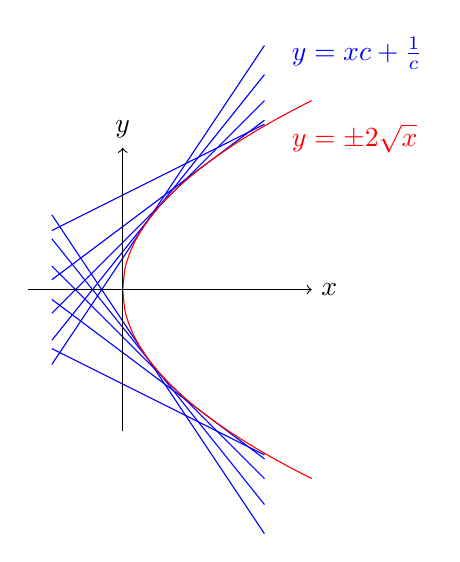
\begin{tikzpicture}[scale=0.6]
  % Curves
  \foreach \c in {-1.5,-1.25,-1,-0.75,-0.5,0.5,0.75,1,1.25,1.5} {
    \draw[blue, domain=-1.5:3] plot (\x, {\x*\c + 1/\c});
  }
  % Envelope
  \draw[red, domain=0:4, smooth, samples=100] plot (\x, {2*sqrt(\x)});
  \draw[red, domain=0:4, smooth, samples=100] plot (\x, {-2*sqrt(\x)});
  % Axis
  \draw[->] (-2,0) -- (4,0) node[right] {$x$};
  \draw[->] (0,-3) -- (0,3) node[above] {$y$};
  % Labels
  %\foreach \c in {5,10} {
   % \draw (\c/5, -0.1) -- (\c/5, 0.1) node[above] {$\c$};
  %}
  \draw (2.2,5) node[right,blue] {$\qquad y=xc+\frac{1}{c}$};
  \draw (2.2,3.2) node[right,red] {$\qquad y=\pm 2\sqrt{x}$};
\end{tikzpicture}$$
\end{sol}
\begin{ejer}
    \textbf{28.} Calcular las soluciones singulares de la ecuación
    $$x-y=\dfrac{4}{9} (y')^2 - \dfrac{8}{27}(y')^3$$
    \textcolor{red}{MAL}
\end{ejer}
\begin{sol}
Planteamos la curva $p$-discriminante
$$\left\{ \begin{array}{l}
     x-y=\dfrac{4}{9}p^2-\dfrac{8}{27}p^3  \\
     \vspace{-5mm} \\
      0=\dfrac{8}{9}p-\dfrac{24}{27}p^2 \; \Rightarrow \; p\left(\dfrac{8}{9}-\dfrac{24}{27}p\right)=0 \; \iff \; \left\{ \begin{array}{ll}
           p=0  \; \Rightarrow \; y=c & \; (1) \\
           \vspace{-5mm}\\ 
            p=\dfrac{8}{9} \cdot \dfrac{27}{24}=\dfrac{216}{216}=1 \; \Rightarrow \; y=x & \; (2)
      \end{array}\right.
\end{array} \right.$$
de forma que, usando (1) en la primera ecuación $x-c=0 \; \Rightarrow \; x=c$ y usando la (2) obtenemos una identidad, luego es solución. Así pues, la única solución singular sería $y=x$. Sea $(x_o,y_o)=(x_o,x_o)$, veamos si para cada punto existe una solución con la misma tangente, es decir, si existe $c$ tal que ambas soluciones ($y=c$ e $y=x$) pasan por el punto y tienen la misma tangente:
$$\left\{ \begin{array}{l}
        x_o=c \: \checkmark \\
        \vspace{-5mm} \\
        0=0 \: \checkmark
    \end{array} \right.$$
   luego la solución singular es $y=x$.
\end{sol}
\begin{ejer}
    \textbf{34.b)} Resolver el sistema:
    $$\left\{ \begin{array}{l}
          \dfrac{dx}{dt}=x \cdot \cos(t) \\
        \vspace{-5mm} \\
          \dfrac{dy}{dt}=\dfrac{(e^t+e^{-t})y}{2}=\dfrac{y}{2}\cdot \cosh(t)
    \end{array} \right.$$
\end{ejer}
\begin{sol}
    $$\left\{ \begin{array}{l}
          \dfrac{dx}{dt}=x \cdot \cos(t) \; \iff \; \dfrac{dx}{x}-\cos(t)dt=0 \; \iff \; \log|x|+\sin(t)=c_1 \; \iff \; x=k_1 e^{-\sin(t)} \\
        \vspace{-5mm} \\
          \dfrac{dy}{dt}=\dfrac{(e^t+e^{-t})y}{2}=y \cdot \cosh(t) \; \iff \;  \: \dfrac{dy}{y}-\cosh(t)dt=0 \; \iff \; \log|y|-\sinh(t)=c_2\; \iff \;  \\
          \hspace{1cm} \iff \; y=k_2\cdot e^{\sinh(t)} 
    \end{array} \right.$$
    Luego las soluciones son
    $$\left\{ \begin{array}{ll}
         x=k_1 \cdot e^{-\sin(t)} & \; \qquad k_1 \in \mathbb R^+\\
         y=k_2 \cdot e^{\sinh(t)}  & \; \qquad \overline{k}_2 \in \mathbb R^+
    \end{array}\right.$$
\end{sol}
\begin{ejer}
     Considérese la ecuación diferencial de segundo orden $y''=-y$. Introduciendo una nueva incógnita, $v$, que haga el papel de $y'$, deducir que dicha ecuación de segundo orden es equivalente a un sistema de dos ecuaciones diferenciales (de primer orden). Sabiendo que $y=\cos(x)$ e $y=\sen(x)$ son dos soluciones de $y''=-y$, obtener todas las soluciones del sistema (y, por tanto, todas las de $y''=-y$).
\end{ejer}
\begin{sol}
    Introduciendo la incógnita $v=y'$, tenemos $v'=y''=-y$ luego el sistema es
    $$\left\{ \begin{array}{ll}
         y'=v & \; \\
         \vspace{-5mm} \\
         v'=-y  & \; 
    \end{array} \right. \iff \left\{ \begin{array}{ll}
         \dfrac{dy}{dx}=v  \\
         \vspace{-5mm} \\
         \dfrac{dv}{dx}=-y \; \Rightarrow \; \dfrac{d}{dx}y'=y''=-y
    \end{array} \right.$$
    Sabiendo que $y_1=\cos(x)$ e $y_2=\sen(x)$ son dos soluciones de $y''=-y$, su suma lo es (por ser sistema lineal homogéneo), y su multiplicación por escalares también, entonces 
    $$y_3=\lambda_1 \cos(x) + \lambda_2 \sen(x)$$ es solución, y por tanto, 
    $$v_3=y_3'=-\lambda_1 \sin(x)+\lambda_2\cos(x)$$
    siendo entonces las soluciones
    $$\begin{pmatrix}
        y\\
        v
    \end{pmatrix}=\begin{pmatrix}
        \cos x & \sin x \\
        -\sin x & \cos x
    \end{pmatrix}\begin{pmatrix}
        \lambda_1\\
        \lambda_2
    \end{pmatrix}$$
    que como hemos visto en el \hyperref[30f]{\textbf{Ejercicio 30.f)}}, las soluciones la ecuación coinciden con las del sistema. 
\end{sol}
\begin{ejer}
    Convertir el sistema de ecuaciones del problema 33 en un sistema de primer orden (añadiendo una nueva incógnita como en el ejercicio anterior).
    $$\left\{ \begin{array}{l}
         x'' = -11x + 4y  \\
         y' = 15x + 6y
    \end{array}\right.$$
\end{ejer}
\begin{sol}
Sea $x'=p$
    $$\left\{ \begin{array}{l}
         x'' = -11x + 4y  \\
         y' = 15x + 6y
    \end{array}\right. \iff \left\{ \begin{array}{l}
         x' = p \\
         p' = -11x+4y\\
         y' = 15x + 6y
    \end{array}\right. \longleadsto{0.5} \begin{pmatrix}
        x' \\ p' \\ y'
    \end{pmatrix}=\begin{pmatrix}
        0 & 1 & 0 \\
        -11 & 0 & 4 \\
        15 & 0 & 6
    \end{pmatrix} \begin{pmatrix}
        x \\ p \\ y 
    \end{pmatrix}$$
\end{sol}
\begin{ejer}
    Comprobar que la función $x^2+y^2$ se mantiene constante en las soluciones de $x'=y$, $y'=-x$ ($x$ e $y$ son funciones incógnitas, dependiente de la variable independiente $t$).
\end{ejer}
\begin{sol}
    Veamos que se mantiene constante, es decir, que $\frac{d}{dt}(x^2+y^2)=0$. Así pues
    $$\dfrac{d}{dt}(x^2(t)+y^2(t))=\dfrac{d(x^2(t))}{dt}+\dfrac{d(y^2(t))}{dt}=2xx'+2yy'$$
    sustituyendo las soluciones $x'=y$ e $y'=-x$:
    $$2xx'+2yy'=2xy+2(-yx)=0$$
    demostrando así que se mantiene constante en las soluciones mencionadas. 
\end{sol}
\begin{ejer}
     Idem para la función $x+y+z$ y el sistema de ecuaciones del problema 36:
     $$\dfrac{dx}{z-y}=\dfrac{dy}{x-z}=\dfrac{dz}{y-x}$$
\end{ejer}
\begin{sol} Véase que equivale al sistema 
    $$\begin{cases} \dfrac{dx}{z-y}=\dfrac{dy}{x-z} \\ \vspace{-5mm} \\ \dfrac{dy}{x-z}=\dfrac{dz}{y-x} \end{cases} \iff \begin{cases} \dfrac{dx}{dy}=\dfrac{z-y}{x-z} \\ \vspace{-5mm} \\ \dfrac{dz}{dy}=\dfrac{y-x}{x-z} \end{cases}$$
    Así pues, comprobemos que es constante
    $$\dfrac{d}{dy}(x+y+z)=\dfrac{dx}{dy}+\dfrac{dy}{dy}+\dfrac{dz}{dy}=\dfrac{z-y}{x-z}+1+\dfrac{y-x}{x-z}=\dfrac{\cancel{z}-\cancel{y}+\cancel{x}-\cancel{z}+\cancel{y}-\cancel{x}}{x-z}=0$$
    luego se mantiene constante.
\end{sol}
\begin{ejer}
    Buscar una función $f(x,y,z)$ que se mantenga constante en las soluciones del problema 38-a (Indicación: buscar entre las funciones simétricas de $x,y,z$):
    $$\left\{ \begin{array}{l}
         \dfrac{dy}{dx}=\dfrac{y(z-x)}{x(y-z)}  \\
         \vspace{-5mm} \\
         \dfrac{dz}{dx}=\dfrac{z(x-y)}{x(y-z)} 
    \end{array} \right.$$
\end{ejer}
\begin{sol}
    La función debe verificar $\frac{d}{dx}f(x,y,z)=0$ y como se indica buscar en las funciones simétricas, estas son
    $$s_1(x,y,z)=x+y+z \qquad s_2(x,y,z)=xy+xz+yz \qquad s_3(x,y,z)=xyz$$
    Comprobemos con $f=s_3$:
    $$\dfrac{d}{dx}(xyz)=yz+x\dfrac{d}{dx}(yz)=yz+x\dfrac{dy}{dx}z+xy\dfrac{dz}{dx}=yz+xz\dfrac{y(z-x)}{x(y-z)}+xy\dfrac{z(x-y)}{x(y-z)}= $$
    $$=yz+\dfrac{xyz^2-\cancel{x^2yz}+\cancel{x^2yz}-xy^2z}{xy-xz}=\dfrac{\cancel{xy^2z}-\cancel{xyz^2}+\cancel{xyz^2}-\cancel{xy^2z}}{xy-xz}=0$$
    Luego $f(x,y,z)=xyz$
\end{sol}
\section{Seminario 6}
\begin{ejer}
    \textbf{30.} Resolver los siguientes sistemas lineales con coeficientes constantes:
    
    $a) \; \left\{ \begin{array}{l}
         \dfrac{dx}{dt}=3x-\dfrac{1}{2}y-3t^2-\dfrac{1}{2}t+\dfrac{3}{2}  \\
         \vspace{-5mm} \\
         \dfrac{dy}{dt}=2y-2t-1
    \end{array} \right.$
    \begin{sol} El sistema es
        $$\begin{pmatrix}
            x' \\ y'
        \end{pmatrix}=\begin{pmatrix}
            3 & -\nicefrac{1}{2} \\
            0 & 2
        \end{pmatrix}\begin{pmatrix}
            x \\ y
        \end{pmatrix}+\begin{pmatrix}
            -3t^2-\nicefrac{1}{2}t+\nicefrac{3}{2} \\ -2t-1
        \end{pmatrix}$$

        \underline{Homogénea}
        $$Y=e^{At}C=B e^{Jt} B^{-1} C=B e^{(D+N)t} B^{-1} C=B e^{Dt} e^{Jt} B^{-1} C$$
        donde $c_A(x)=6-5x+x^2=(x-3)(x-2)$, luego $J=\begin{pmatrix}
            3 & 0 \\
            0 & 2
        \end{pmatrix}=D+\cancel{N}=D$ $$\begin{pmatrix}
            x \\ y
        \end{pmatrix}=\begin{pmatrix}
            \nicefrac{1}{2} & 1 \\
            1 & 0
        \end{pmatrix}\begin{pmatrix}
            e^{3t} & 0 \\
            0 & e^{2t}
        \end{pmatrix}\begin{pmatrix}
            0 & 1 \\
            1 & \nicefrac{1}{2} 
        \end{pmatrix}\begin{pmatrix}
            c_1 \\ c_2
        \end{pmatrix} =\begin{pmatrix}
            \nicefrac{e^{2t}}{2} & e^{3t} \\ e^{2t} & 0
        \end{pmatrix}\begin{pmatrix}
            0 & 1 \\
            1 & \nicefrac{1}{2} 
        \end{pmatrix}\begin{pmatrix}
            c_1 \\ c_2
        \end{pmatrix}= \begin{pmatrix}
            e^{3t} & \nicefrac{1}{2}(e^{2t}-e^{3t}) \\ 0 & e^{2t} 
        \end{pmatrix}\begin{pmatrix}
            c_1 \\ c_2
        \end{pmatrix}$$
    \end{sol}

    \underline{Particular}
    $$\begin{pmatrix}
            x_p \\ y_p
        \end{pmatrix}= \begin{pmatrix}
            e^{3t} & \nicefrac{1}{2}(e^{2t}-e^{3t}) \\ 0 & e^{2t} 
        \end{pmatrix}\begin{pmatrix}
            c_1(t) \\ c_2(t)
        \end{pmatrix} \text{ con } e^{At}C'(t)=\begin{pmatrix}
            -3t^2-\nicefrac{1}{2}t+\nicefrac{3}{2} \\ -2t-1
        \end{pmatrix} $$$$\; \iff \; C'(t)=e^{-At}\begin{pmatrix}
            -3t^2-\nicefrac{1}{2}t+\nicefrac{3}{2} \\ -2t-1
        \end{pmatrix} =\begin{pmatrix}
            e^{-3t} & \nicefrac{1}{2}(e^{-2t}-e^{-3t}) \\ 0 & e^{-2t} 
        \end{pmatrix}\begin{pmatrix}
            -3t^2-\nicefrac{1}{2}t+\nicefrac{3}{2} \\ -2t-1
        \end{pmatrix}$$
        $$\begin{pmatrix}
            x_p \\ y_p
        \end{pmatrix}=\begin{pmatrix}
            t^2+t \\ t+1
        \end{pmatrix}$$

    $b) \; \dfrac{dx}{dt}+5x+y=e^t, \; \dfrac{dy}{dt}-x+3y=e^{2t}$
    \begin{sol}
        
    \end{sol}
    $c) \; \dfrac{dx}{dt}=y, \; \dfrac{dy}{dt}=z, \; \dfrac{dz}{dt}=x$
    \begin{sol}
        $$\begin{pmatrix}
            x' \\ y' \\ z'
        \end{pmatrix}=\begin{pmatrix}
            0 & 1 & 0 \\
            0 & 0 & 1 \\
            1 & 0 & 0 
        \end{pmatrix}\begin{pmatrix}
            x \\ y \\ z
        \end{pmatrix} \; \Rightarrow \; \begin{pmatrix}
            x \\ y \\ z 
        \end{pmatrix}=e^{tA}C$$
        con el cambio de base
        $$A=\begin{pmatrix}
            1 & \alpha & \alpha^2 \\ 1 & \alpha^2 & \alpha \\ 1 & 1 & 1
        \end{pmatrix}\begin{pmatrix}
            1 & \\ & \alpha \\ & & \overline{\alpha}
        \end{pmatrix}\begin{pmatrix}
            1 & \alpha & \alpha^2 \\ 1 & \alpha^2 & \alpha \\ 1 & 1 & 1
        \end{pmatrix}^{-1} \qquad \alpha=\dfrac{-1+\sqrt{3}i}{2} \quad \overline{\alpha}=\dfrac{-1-\sqrt{3}i}{2}$$
        y finalmente obtenemos
    \end{sol}
\end{ejer}
\begin{ejer}
    \textbf{32.} Resolver el sistema
    $$\dfrac{dx}{3x-y}=\dfrac{dy}{x+y}=\dfrac{dz}{3x+5y-3u}=\dfrac{du}{4x-y+3z-u}$$
    introduciendo una variable auxiliar $t$ e igualando los términos anteriores a $dt$, con
lo que el sistema es lineal homogéneo con coeficientes constantes.
\end{ejer}
\begin{ejer} \textbf{33.}
    Introduciendo una nueva incógnita, integrar el sistema siguiente reduciéndolo a
uno de primer orden:
$$\left\{ \begin{array}{l}
         x''=-11x+4y \\
        y'=15x+6y
    \end{array}\right.$$
\end{ejer} 
\begin{sol}
    La matriz asociada al sistema, como vimos en el seminario anterior es 
    $$A=\begin{pmatrix}
        0 & 1 & 0 \\
        -11 & 0 & 4 \\
        15 & 0 & 6
    \end{pmatrix}$$
    y la solución es $Y=e^{At} C$ donde la descomposición de Jordan de la matriz es
    $$ A=B J B^{-1} $$ 
    luego 
    $$Y=B e^D \cancel{e^J} B^{-1} C=B e^D B^{-1} C$$
    
\end{sol}
\begin{ejer}
    \textbf{43.} Resolver las siguientes ecuaciones diferenciales

    $c) \; yy''+(y')^2 = 0$
        \begin{sol}
    Haciendo $p=y'$, hagamos 
    $$\dfrac{dp}{dy}=\dfrac{\nicefrac{dp}{dx}}{\nicefrac{dy}{dx}}=\dfrac{y''}{p} \; \Rightarrow \; y''=p \dfrac{dp}{dy}$$
y sustituyendo en la ecuación original
$$y \cdot p \dfrac{dp}{dy}+p^2=0  \; \iff \; p\left( y \cdot \dfrac{dp}{dy}+p=0\right) \; \iff \; \left\{ \begin{array}{l}
     p = 0 \; \iff \; y'=0 \; \iff \; y=c  \\
     \vspace{-5mm} \\
     y \dfrac{dp}{dy}+p=0 \; \iff \; \dfrac{dp}{p}+\dfrac{dy}{y}=0 \; \iff \; p=-cy  \\
     \qquad \qquad \quad \iff \; y'=-cy \; \iff \; \boxed{ \: y=c_2\cdot e^{-cx} \: }
\end{array}\right.$$
\end{sol}

    $d) \; (y'')^2 + x^2 = 1$
\begin{sol}
    Consideramos $z=y'$, entonces la ecuación es $(z')^2+x^2=1$, que parametrizada es
    $$\left\{ \begin{array}{l}
         x=\cos t  \\
         z'=\sin t  
    \end{array} \right.$$
    y por la regla de la cadena, 
    $$\sin t =z'=\dfrac{dz}{dx}=\dfrac{\nicefrac{dz}{dt}}{\nicefrac{dx}{dt}}=\dfrac{\nicefrac{dz}{dt}}{-\sin t} \; \Rightarrow \; \dfrac{dz}{dt}=-\sin^2 t = -\left( \dfrac{1-\cos 2t}{2}\right)$$
    e integrando, 
    $$z=-\dfrac{1}{2}t+\dfrac{1}{4} \sin 2t + c_1$$
    y recuperando el cambio de variable,
    $$z(t)=y'=\dfrac{\nicefrac{dy}{dt}}{\nicefrac{dx}{dt}}=\dfrac{\nicefrac{dy}{dt}}{-\sin t} \;\Rightarrow \; \dfrac{dy}{dt}=-\sin t\left( -\dfrac{1}{2}t+\dfrac{1}{4}\sin 2t+c_1\right)=\dfrac{1}{2}t \sin t - \dfrac{1}{2} \sin^2 t \cos t - c_1\sin t$$
    e integrando
    $$y=\dfrac{1}{2}(-t \cos t+\sin t )- \dfrac{1}{2}\dfrac{\sin^3 t}{3}+c_1\cos t +c_2$$
    y sustituyedo $x=\cos t$ tendríamos la solución expresada como buscamos.
\end{sol}
    $g) \; (y''')^2+(y'')^2=1$
\begin{sol}
Llamamos $u:=y''$, y parametrizamos la circunferencia
    $$\left\{ \begin{array}{l}
         u=\cos t  \\
         u'=\sin t  
    \end{array} \right.$$
    y al igual que en el ejercicio anterio


    Hacemos $z=(y'')^2$, de forma que tenemos 
    $$z'=2y''y''' \; \Rightarrow \; (y''')^2=\left(\dfrac{z'}{2y''}\right)^2=\dfrac{(z')^2}{4(y'')^2}=\dfrac{(z')^2}{4z}$$
    y la ecuación es 
    $$\dfrac{(z')^2}{4z}+z=1 \; \iff \; (z')^2-4z+4z^2=0 \; \iff \; z'=\sqrt{4z-4z^2}=2\sqrt{z(1-z)} \; \iff$$
    $$\iff \; z=\dfrac{1}{4} \sqrt{-((-1 + z) z)} (-1 + 2 z) - \arcsin(\sqrt{1 - z})$$
\end{sol}
\end{ejer}
\section{Seminario 7}
\begin{ejer}
    \textbf{45.}c) $y^{(4} - 16y = x^4+x+1$
\end{ejer}
\begin{sol}
    La ecuación es equivalente a $(D^4-16y=x^4+x+1)$. Resolvemos la homogénea:

    \underline{Homogénea} $(D^4-16)y=0$
    $$D^4-16=(D^2+4)(D-2)(D+2) \; \Rightarrow \; \ker (D^4 +16)=\ker (D^2+4) \oplus \ker (D-2) \oplus \ker(D+2)=$$
    $$=<\cos(2x),\sin(2x)>\oplus <e^{-2x}> \oplus <e^{2x}> \;\Rightarrow \; y_h=<\cos(2x),\sin(2x) , e^{-2x} , e^{2x}> =$$
    $$=\{ c_1 \cos(2x) + c_2 \sin(2x) +c_3 e^{-2x}> +c_4 e^{2x}>$$

    \underline{Particular}

    Por el método del anulador, buscamos un polinomio de grado 5 primo con $b(x)=x^4+x+1$, sea $Q(D)=D^5$, 
    $$D^5=(D^4-16)D + 16D$$
    y por el Algoritmo de Euclídes, 
    $$y_p=A(D)b(x)=-\dfrac{1}{16}\left(x^4+x+1+\dfrac{24}{16} \right)$$
\end{sol}
\begin{ejer} \textbf{39.}
    Calcular 2 integrales $1^{as}$ independientes del campo
    $$D=\pd{}{t}+(2x-5y)\pd{}{x}+(2x-4y)\pd{}{y}$$
    como campo en $\mathbb R^3_{t,x,y}$.
\end{ejer}
\begin{sol}
    Ponemos el sistema equivalente:
    $$dt=\dfrac{dx}{2x-5y}=\dfrac{dy}{2x-4y} \; \iff \; \left\{ \begin{array}{l}
         \dfrac{dx}{dt}=2x-5y  \\
         \vspace{-5mm} \\
          \dfrac{dy}{dt}=2x-4y
    \end{array}\right.\longleadsto{0.5} \dfrac{d}{dt}\begin{pmatrix}
        x \\ y 
    \end{pmatrix}=\begin{pmatrix}
        2 & -5 \\ 2 & -4 
    \end{pmatrix} \begin{pmatrix}
        x \\ y 
    \end{pmatrix}$$
    luego como para todos los sistemas,
    $$\begin{pmatrix}
        x \\ y 
    \end{pmatrix} = e^{\left(\begin{smallmatrix}
       2 & -5 \\ 2 & -4 
    \end{smallmatrix}\right)t} \begin{pmatrix}
        c_1\\ c_2 
    \end{pmatrix}$$
    de forma que las integrales primeras son 
    $$ \begin{pmatrix}
        c_1\\ c_2 
    \end{pmatrix} = e^{-\left(\begin{smallmatrix}
       2 & -5 \\ 2 & -4 
    \end{smallmatrix}\right)t} \begin{pmatrix}
        x \\ y 
    \end{pmatrix}= \begin{pmatrix}
        \alpha(t,x,y) \\ \beta(t,x,y) 
    \end{pmatrix}$$
    siendo $ \alpha(t,x,y)$ y $ \beta(t,x,y)$ las integrales $1^{as}$
\end{sol}
\begin{ejer}
    \textbf{58.} Calcular la solución de $x\pd{z}{y}=z$ que pase por la curva $y=2, z=x$.
\end{ejer}
\begin{sol}
    $$\pd{z}{y}=\dfrac{z}{x} \; \Rightarrow \; D=\pd{}{y} \; \Rightarrow \; x \text{ es integral 1ª} \; \Rightarrow \; z=e^{\nicefrac{1}{x} y} \cdot \varphi(x) \qquad \varphi \text{ arbitraria.}$$
    Imponemos que dicha solucón (superifie) pase por la curva dada, determinando así $\varphi$. Podemos reescribir la curva como
    $$\left\{ \begin{array}{l}
         x=t  \\
         y=2 \\
         z=t
    \end{array} \right.$$
    y sutituimos en la solución:
    $$z=e^{\nicefrac{1}{x} y} \cdot \varphi(x) \; \Rightarrow \; t=e^{\nicefrac{2}{t}}\varphi(t) \; \iff \; \varphi(t)=t e^{-\nicefrac{2}{t}}$$
    y sutituyendo en la ecuación, la solución buscada es
    $$z=e^{\frac{1}{x} y} \cdot x e^{-\nicefrac{2}{x}} \qquad x \neq 0 $$
\end{sol}
\begin{ejer}
    \textbf{inventao.} Calcular la solución de $$-y \pd{z}{x} + x \pd{z}{y}=(x^2+y^2)z$$ que pase por la curva $x=y,\: z=x^2$.
\end{ejer}
\begin{sol}
    Consideramos el campo 
    $$D=-y \pd{z}{x} + x \pd{z}{y}$$
    y con ese campo la ecuación es $Dz=(x^2+y^2)$. Reducimos $D$ a la forma canónica, sabiendo que es el de los giros, en coordenadas polares,
    $$\left\{ \begin{array}{l}
         r=\sqrt{x^2+y^2}  \\
         \theta=arg(x,y) 
    \end{array}\right. \; \Rightarrow \left\{ \begin{array}{l}
        Dr=0  \\
        D\theta=-y \pd{arg(x,y)}{x}+x\pd{arg(x,y)}{y}
    \end{array}\right.$$ 
    de forma que 
    $$\pd{arg(x,y)}{x}=\pd{\arctan(\nicefrac{y}{x})}{x}=\dfrac{-\nicefrac{y}{x^2}}{1+\left(\nicefrac{y}{x}\right)^2}=\dfrac{-y}{x^2+y^2} \qquad \pd{arg(x,y)}{y}=\dfrac{\cos \theta}{r}=\dfrac{x}{x^2+y^2}$$
    y por tanto $$D\theta = -y \dfrac{-y}{x^2+y^2} + x \dfrac{x}{x^2+y^2}=1$$
    luego 
    $$\boxed{D=\pd{}{\theta}}$$
    La ecuación entonces se escribe como
    $$\pd{z}{\theta}=r^z \; \Rightarrow \; z=e^{r^2 \theta} \varphi(r) \equiv  z=e^{(x^2+y^2) arg(x,y)} \varphi(\sqrt{x^2+y^2}) $$
    Imponemos el paso por la curva $\{x=t,y=t,z=t^2\}$, de forma que
    $$t^2=e^{2t^2 arg(t,t)} \varphi(\sqrt{2}t) \; \Rightarrow \;  \varphi(\sqrt{2}t)=t^2 e^{-2t^2arg(t,t)}$$
    y haciendo el cambio $s=\sqrt{2}t$, 
    $$\varphi(s)=\dfrac{s^2}{2} e^{-s^2arg\left(\nicefrac{s}{\sqrt{2}},\nicefrac{s}{\sqrt{2}}\right)}$$ 
    y sustituyendo en la solución
    $$z=e^{(x^2+y^2) arg(x,y)} \varphi(\sqrt{x^2+y^2}) \; \Rightarrow \; z=e^{(x^2+y^2) arg(x,y)} \dfrac{x^2+y^2}{2} \: e^{-(x^2+y^2)\nicefrac{\pi}{4}}$$
\end{sol}
\section{Seminario 8}
\begin{ejer}[\textbf{53}.a] Calcular los cuatro primeros términos del desarrollo en serie de potencias centrado
    en $x_o = 0$ de la solución del siguiente problema de Cauchy:
    $$\left\{ \begin{array}{l}
     y'' + 3xy' - y = 0 \\
     y(0) = 2 \\
     y'(0) = 0
\end{array}\right.$$
\end{ejer}
\begin{ejer}[\textbf{54}.a] Calcular la solución general de la siguiente ecuación mediante desarrollos en serie de potencias generalizadas en un entorno del punto singular regular $x_o = 0$:
$$(x + 2)x^2y'' - xy' + (1 + x)y = 0, \;  x > 0$$
\end{ejer}
\begin{ejer}[\textbf{55}] Para cada $\alpha \in  \mathbb R$, probar que la serie $y := \sum_{m\geq 0}{\alpha \choose m} x^m$ es convergente en $|x| < 1$ y satisface el problema de condiciones iniciales $(1 + x)y' = \alpha y, \: y(0) = 1$. Deducir, para $|x| < 1$, el desarrollo binomial:
    $$(1+x)^{\alpha}= \sum_{m\geq 0}{\alpha \choose m} x^m$$
\end{ejer}
\begin{sol}
    Definamos el término general de la serie, que es $a_n={\alpha \choose n}$.
    Para demostrar que el radio de convergencia es 1, veamos cual es el siguiente límite:
    $$L=\lim_{n \to \infty} \left|\dfrac{a_{n+1}}{a_n}\right|=\lim_{n \to \infty} \left|\dfrac{{\alpha \choose n+1}}{{\alpha \choose n}}\right|=\lim_{n \to \infty} \left|\dfrac{\frac{\cancel{\alpha!}}{(m+1)!(\alpha-(m+1))!}}{\frac{\cancel{\alpha!}}{m!(\alpha-m)!}}\right|=\lim_{n \to \infty} \left|\dfrac{\cancel{m!}(\alpha-m)!}{(m+1)\cdot \cancel{m!}(\alpha-(m+1))!}\right|= $$
    $$=\lim_{n \to \infty} \left|\dfrac{(\alpha-m)\cancel{(\alpha-m-1)!}}{(m+1)\cancel{(\alpha-m-1)!}}\right|=\lim_{n \to \infty} \left|\dfrac{\alpha-m}{m+1}\right| =\lim_{n \to \infty} \left|\dfrac{\alpha}{m+1}-\dfrac{m}{m+1}\right|=\lim_{n \to \infty} \left|\cancelto{0}{\dfrac{\alpha}{m+1}}- \dfrac{m}{m+1}\right|= $$
    $$=\lim_{n \to \infty}\left|-\dfrac{\nicefrac{m}{m}}{\nicefrac{m}{m}+\nicefrac{1}{m}}\right|=\lim_{n \to \infty}\left|- \dfrac{1}{1+\cancelto{0}{\nicefrac{1}{m}}}\right|=|-1|=1$$
    Luego el radio de convergencia es $R=\nicefrac{1}{L}=1$. 
        
    Veamos si satisface el problema. Dado que $y=(1+x)^{\alpha}$, $y'=\alpha(1+x)^{\alpha-1}$, y por tanto, 
    $$(1 + x)y' = \alpha y \iff (1+x)\alpha(1+x)^{\alpha-1}=\alpha (1+x)^{\alpha} \iff \alpha (1+x)^{\alpha}=\alpha (1+x)^{\alpha} \checkmark $$
    y $1=y(0)=(1+0)^{\alpha}=1^{\alpha}=1$, por lo que también se verifica. 
\end{sol}

\section{Seminario 9}
\begin{ejer}[\textbf{59}] Integrar
    $$z\pd{z}{x}- y\pd{z}{y} = 0$$
\end{ejer}
\begin{sol}
    Su campo asociado es 
    $$D=z \pd{}{x} + y\pd{}{y} + 0\pd{}{z} $$
    y buscamos sus integrales $1^{as}$:
    $$ \left\{ \begin{array}{l}
     \dfrac{dx}{\lambda}=\dfrac{dy}{y} \; \Rightarrow \; \dfrac{x}{\lambda}=\ln|y|+\mu \; \Rightarrow \; \mu=\nicefrac{x}{z}-\ln|y| \text{ Integral 1ª} \\  
     \vspace{-5mm} \\
    \dfrac{dz}{dt}=0 \; \Rightarrow \; z=:\lambda \text{ Integral 1ª}\\
     \vspace{-5mm} \\
\end{array}\right.$$
y uniendo las dos primeras, $x=\mu \ln|y|$, luego $\mu=\nicefrac{x}{\ln|y|}$ es otra integral 1ª. De esta forma, expresamos el campo en coordenadas $x, \mu,\lambda=z$ y por tanto, 
$$D=Dx \pd{}{x} = z \pd{}{x} \; \Rightarrow \; Dz=0$$
luego $Dz=0$. De esta forma, cualquier función que sea combinación algebraica de $\lambda, \mu$ es solución despejando la $z$, es decir, 
$$\gamma(\lambda,\mu)=\gamma(z,\nicefrac{x}{z}-\ln|y|)=0 $$
\end{sol}



\begin{ejer}[\textbf{60}] Calcular una solución de 
    $$yz\pd{z}{x}+ \pd{z}{y} = 0$$
    pasando por la curva $x=0, \: z=y^3$.
\end{ejer}
\begin{sol}
    Buscamos la integrales $1^{as}$ del campo $D=yz\pd{}{x}+\pd{}{y} + 0 \pd{}{z}$
    $$\dfrac{dx}{yz}=dy$$
    y como además $\frac{dz}{dt}=0$, $z=\lambda$ es una integral 1ª. Entonces
    $$dx=\mu y dy \; \Rightarrow \; x=\dfrac{\mu}{2} y^2 \; \Rightarrow \; \mu = \dfrac{x}{y^2}$$
    que es otra integral primera. Así, como siempre, cambiamos de coordenadas a $(x,\lambda=z, \mu)$ y el campo es $$D=Dx \pd{}{x} + Dz \pd{}{z} + D\mu \pd{}{\mu}=Dx \pd{}{x}=yz\pd{}{x} \; \Rightarrow \; Dz=0 $$
    y por tanto una solución es la función
    $$z=\alpha\left(\dfrac{x}{y^2}\right)$$
    y para que cumpla las condiciones, parametrizamos la curva, $y=t$, $z=t^3$, $x=0$, de forma que
    $$t^3=\alpha(0)  \; \Rightarrow \; t=0$$
    \textcolor{red}{TERMINAR}
\end{sol}
\begin{ejer}[\textbf{38}] Resolver los sistemas
$$a) \left\{ \begin{array}{l}
     \dfrac{dy}{dx}=\dfrac{y(z-x)}{x(y-z)}\\
     \vspace{-5mm} \\
      \dfrac{dz}{dx}=\dfrac{z(x-y)}{x(y-z)}
\end{array}\right. \qquad b) \left\{ \begin{array}{l}
     \dfrac{dy}{dx}=\dfrac{y(z^2-x^2)}{x(y^2-z^2)}\\
     \vspace{-5mm} \\
      \dfrac{dz}{dx}=\dfrac{z(x^2-y^2)}{x(y^2-z^2)}
\end{array}\right.$$
Para el apartado a) buscar integrales primeras simétricas en $x, y, z$. El apartado
b) se reduce al a) multiplicando la primera ecuación por $y/x$ y la segunda por $z/x$.    
\end{ejer}
\begin{sol}
    Podemos expresar ambas como
    $$\dfrac{dx}{x(y-z)}=\dfrac{dy}{y(z-x)}=\dfrac{dz}{z(x-y)}$$
    es donde buscamos las integrales $1^{as}$ del campo
    $$D=x(y-z)\pd{}{x} + y(z-x)\pd{}{y} + z(x-y) \pd{}{z}$$
    Como toda función simétrica es función de las elementles, elegimos una y probamos. 
\end{sol}
\begin{ejer}
    [\textbf{42}] Hallar un campo que sea tangente a las circunferencias que pasan por el origen y que tienen su centro en el eje de abcisas.
\end{ejer}
\begin{sol}
    Considerando las subvariedades de las circunferencias en $\mathbb R^2$, $S \equiv \{x^2+y^2=r^2\}$ \textcolor{red}{NO SE HIZO}
\end{sol}
\begin{ejer}
    Calcular una solución de la ecuación del ejemplo 7.10 de las notas de teoría (página 38)  pasando por la curva $y=0, x=z^3$ y lo mismo con la curva $x=1$, $y=z^2$. El ejemplo 7.10 es la solución a la ecuación
    $$z \pd{z}{x} + x \pd{z}{y}=xz$$
    \textcolor{red}{NO SE HIZO}
\end{ejer}
\begin{ejer}
    Sea $D$ un campo no nulo en ningún punto. Probar que todas las hipersuperficies tangentes a $D$ se pueden expresar (localmente) con una ecuación $g=0$, donde $g$ es una integral primera de $D$.
\end{ejer}
\begin{sol}
    Localmente, cualquier hipersuperficie ($\dim S=n-1$), es de la forma $S \equiv \{f(x_1,\ldots,x_n)=0\}$ tal que $d_pf\neq 0 \: \forall p \in S$. El problema consiste en probar que $S$ localmente es una integral primera del campo $D$. 

    Solo sabemos que $D_pf=0 \: \forall p \in S$ o equivalentemenete $D_pf=0 \iff f(p)=0$. Podemos hacer un cambio de coordenadas de forma que $f=x_1$, y por tanto $S\equiv\{x_1=0\}$. Además, $Dx_1=0$ cuando $x_1=0$, es decir, $Dx_1=x_1 \cdot h(x_1,\ldots,x_n)$ como hacíamos en Análisis III, integrando por un segmento. 

    Buscamos pues una función $g$ tal que $x_1 \cdot g$ sea integral 1ª. Queremos que se verifique que 
    $$0=D(x_1 \cdot g)=Dx_1 g+ x_1 Dg=x_1( gh + Dg)$$
    y basta con que $Dg=hg$ (siendo $h$ una función dada, se trata de buscar $g$). \textcolor{red}{TERMINAR EXAMEEEEEEN!!!!!!!} Se puede generalizar para subvariedades de dimensión menor.
\end{sol}

\section{Seminario 10}
\begin{ejer} Sea $f$ continua y periódica con $f'$ continua, consideramos $a_n(f)$ y $b_n(f)$, $a_n(f')$ y $b_n(f')$. Se pide relacionar los coeficientes de una y otra. Indicación: integrar por partes y poner en función de $f'$.
    
\end{ejer}
            \begin{sol}
                $$a_n=\int_0^{2 \pi}  \dfrac{f \cdot \cos(nx)}{\sqrt{\pi}} dx=\dfrac{1}{\sqrt{\pi}} \int_0^{2 \pi}  f \cdot \cos(nx) dx= \begin{cases}
                    f(x)=u & f'dx=du \\ dv=\cos(nx) dx & v=\dfrac{-\sin(nx)}{n}
                \end{cases}$$
                luego por la integración por partes
                $$ \dfrac{-(f \cdot \sin(nx))}{\sqrt{\pi}n} - \int \dfrac{-(f' \cdot \sin(nx))}{\sqrt{\pi}n} dx = \dfrac{1}{n\sqrt{\pi}} \left( \cancelto{0}{-(f \cdot \sin(nx))}\Big|_0^{2\pi} - b_k(f')\right)$$
                y de la misma forma
                $$b_k(f)=\dfrac{1}{k} \left(\dfrac{1}{\sqrt{\pi}} \left[ \cancelto{0}{-f(x) \cdot \cos(kx)}\right]_{0}^{2\pi} + a_k(f')\right)=\dfrac{1}{k}a_k(f')$$
            \end{sol}
 \begin{ejer}
 Considerando $f$ continua y periódica, se tienen $f \longleadsto{0.5} S_f \longleadsto{0.5} (S_f)'$ es la derivada de la serie, suponiendo que se puede derivar término a término. También consideramos $f \longleadsto{0.5} f' \longleadsto{0.5} S_{f'}$. Se pide encontrar la relación entre $(S_f)'$ y $S_{f'}$.
 \end{ejer}
 \begin{sol}
     Dada $S_f=a_o+\sum a_k \cos(kx)+b_k \sin(kx)$, entonces usado las identidades anteriores
     $$S_f=a_o(f)\dfrac{1}{\sqrt{2\pi}}+\sum_{k=1}^{\infty} \dfrac{-b_k(f')}{k} \dfrac{\cos(kx)}{\sqrt{\pi}}+ \dfrac{a_k(f')}{k} \dfrac{\sin(kx)}{\sqrt{\pi}}$$
     y derivando
     $$(S_f)'=\sum_{k=1}^{\infty} b_k(f') \dfrac{\sin(kx)}{\sqrt{\pi}} + a_n(f') \dfrac{\cos(kx)}{\sqrt{\pi}} = S_{f'} - a_o(f')\dfrac{1}{\sqrt{2\pi}}$$
 \end{sol}
 \begin{obs}
 Consideremos una función $\mc{C}^0_{trozos}$, es decir, continua a trozos, y existiendo los límites en las discontinuidades. De la misma forma, podemos definir funciones  $\mc{C}^1_{trozos}$, que serán  $\mc{C}^0_{trozos}$ y además existirá los límites laterales de la derivada en las discontinuidades. Podemos además definir funciones $\mc{C}^0$ y $\mc{C}^1_{trozos}$. \textcolor{red}{DIBUJOS}
 \end{obs}
 \begin{ejer}
     Supongamos $f$ del último tipo, que en principio es solo derivable donde no cambia bruscamente la pendiente. En ese caso, $f'$ como función es continua a trozos. Se pide ver si se mantienen las relaciones entre $a_n(f)$ y $b_n(f)$ y los coeficientes de $f'$.
 \end{ejer}
 \section{Seminario 11}
 Los ejercicios propuestos para el seminario son los siguientes:
\begin{enumerate}
    \item Calcular el desarrollo de Fourier de $f : [0, 2\pi] \longrightarrow \mathbb R$, donde $f(x) := \cos(\nicefrac{x}{2})$.
    \begin{sol}
        Dado que es una función par y periódica, bastará calcular los $a_i$. En primer lugar
        $$a_o=\dfrac{1}{\sqrt{2\pi}}\int_0^{2\pi} \cos(\nicefrac{x}{2}) dx = \dfrac{2 \sin(\nicefrac{x}{2})}{\sqrt{2\pi}} \Big|_{0}^{2\pi}=0$$
        y después
        $$a_n=\dfrac{1}{\sqrt{\pi}}\int_0^{2\pi} \cos(\nicefrac{x}{2}) \cos(nx) dx = 0$$
        $$b_n=\dfrac{1}{\sqrt{\pi}}\int_0^{2\pi} \cos(\nicefrac{x}{2}) \sin(nx) dx = \dfrac{8 n }{-1 + 4 n^2}$$
        luego la serie es 
        $$\cos\left(\dfrac{x}{2} \right)=\dfrac{1}{\sqrt{\pi}}\sum_{n=1}^{\infty} \dfrac{8 n }{ 4 n^2-1} \sin(nx)$$
    \end{sol}
    \item Calcular el desarrollo de Fourier de $f(x) := x^2$ en $[0, 2\pi]$ y obtener una expresión para $\pi^4$ utilizando la identidad de Parseval.
    \begin{sol} Los coeficientes son
        $$a_o=T_2(x^2,\nicefrac{1}{\sqrt{2\pi}})= \dfrac{1}{\sqrt{2\pi}} \int_0^{2\pi} x^2 dx=\dfrac{x^3}{3\sqrt{2\pi}} \Big|_0^{2\pi}=\dfrac{8 \pi^3}{\sqrt{8\pi}}=2\sqrt{2\pi^5}$$
            $$a_k=\int_0^{2 \pi} x^2 \dfrac{\cos(kx)}{\sqrt{\pi}} dx = \dfrac{1}{\sqrt{\pi}}\int_0^{2 \pi} x^2 \cos(kx) \: dx = \dfrac{x^2 \sin(kx)}{\sqrt{\pi}k}-\dfrac{1}{\sqrt{\pi}k} \int_0^{2\pi} 2x \sin(kx) dx=$$
            $$= \dfrac{x^2 \sin(kx)}{\sqrt{\pi}k}-\dfrac{1}{\sqrt{\pi}k} \dfrac{2 \sin(k x) - 2 k x \cos(k x)}{k^2} \Big|_{0}^{2\pi} = \dfrac{4k\pi}{k^3 \sqrt{\pi}}=\dfrac{4\sqrt{\pi}}{k^2}$$

            $$b_k=\int_0^{2 \pi}  \dfrac{x^2 \sin(kx)}{\sqrt{\pi}} dx = \dfrac{1}{\sqrt{\pi}} \int_0^{2 \pi}  x^2 \sin(kx) dx = \dfrac{1}{k \sqrt{\pi}} \left( \dfrac{(k^2 x^2 - 2) \sin(k x) + 2 k x \cos(k x)}{k^3}dx\right|_0^{2\pi}=$$
            $$=\dfrac{4k\pi}{k^4\sqrt{\pi}}=\dfrac{4\sqrt{\pi}}{k^3}$$
            y por tanto, la serie es 
            $$x^2=\dfrac{2\sqrt{2\pi^5}}{\sqrt{2\pi}} + \mathlarger{\sum}_{k=1}^{\infty} \dfrac{4}{k^2} \cos(kx) + \dfrac{4}{k^3} \sin(kx)= 2\pi^2 + 4 \mathlarger{\sum}_{k=1}^{\infty} \dfrac{\cos(kx)}{k^2} + \dfrac{\sin(kx)}{k^3}$$
            y usando la identidad de Parceval
            $$\|x^2\|^2\underset{P.}{=}a_o^2 + \sum_{k\geq 1} a_k^2 + b_k^2 = 8\pi^5 + 16 \sum_{k\geq 1} \dfrac{1}{k^4} + \dfrac{1}{k^6} =8\pi^5 + 16 \sum_{k\geq 1} \dfrac{1}{k^4} + \sum_{k\geq 1} \dfrac{1}{k^6} $$
            donde 
            $$\|x^2\|^2=\int_0^{2\pi} x^2 dx= \dfrac{x^3}{3} \Big|_0^{2\pi}=\dfrac{2}{3} \: \pi^3$$
            y por tanto:
            $$\dfrac{2}{3} \: \pi^3= 8\pi^5 + 16 \sum_{k\geq 1} \dfrac{1}{k^4} + \dfrac{1}{k^6}$$
            lo cual equivale a 
            $$\dfrac{2/3\pi^3- 8\pi^5}{16}=\pi^3\left(\dfrac{1}{24}-\dfrac{1}{2}\pi^2\right)= \: \sum_{k\geq 1} \dfrac{1}{k^4} + \dfrac{1}{k^6} $$
            
    \end{sol}
    \item Calcular el desarrollo de Fourier en senos de la función $\phi: [0, \pi] \longrightarrow \mathbb R$, dada por $\phi(x) := x^2$.
    \begin{sol}
        Para calcular el desarrollo en senos, debemos extenderla imparmente periódicamente, de forma que es
        $$\hat{\phi}(x)=\left\{ \begin{array}{ll} -x^2 & \text{ en } [-\pi,0]+2\pi n \\ x^2 & \text{ en } [0, \pi]+2\pi n
        \end{array} \right. \forall n \in \mathbb N$$
        y el coeficientes es
        \begin{equation*}\begin{split}
        b_n&= \dfrac{1}{\sqrt{\pi}} \int_{-\pi}^{\pi} \hat{\phi} \sin(nx) dx =\dfrac{1}{\sqrt{\pi}} \int_{-\pi}^{\pi}\hat{\phi} \sin(nx) dx +\int_{\pi}^{2\pi} \hat{\phi} \sin(nx) dx = \\
         &=\dfrac{1}{\sqrt{\pi}} \int_0^{\pi} \hat{\phi} \sin(nx) dx +\int_{-\pi}^{0} \hat{\phi} \sin(nx) dx =\dfrac{1}{\sqrt{\pi}} \int_0^{\pi} x^2 \sin(nx) dx +\int_{-\pi}^{0} -x^2 \sin(nx) dx= \\
         &=\dfrac{-2\pi^2}{n\sqrt{\pi}} =-\dfrac{2\sqrt{\pi^3}}{n} 
        \end{split}           
        \end{equation*}
        $$S_{\hat{\phi}}=-2\pi\sum \dfrac{\sin(nx)}{n} $$
    \end{sol}
    \item Idem para $\psi: [0, 10] \longrightarrow \mathbb R$, $\psi(x) := x$.
    \begin{sol}
        Hacemos la extensión impar, de forma que $\hat{\psi}$ debe ser de periodo 20=2$\cdot$10, y se tiene
        $$\hat{\psi}(x)= x + 20n\text{ en } [-10,10]\forall n \in \mathbb N$$
        ya que ya es impar, solo es convertirla en periódica de periodo $20$. Entonces, 
        \begin{equation*}\begin{split}
        b_n&=\dfrac{1}{\sqrt{\pi}} \int_{-10}^{10} \hat{\psi}(x) \sin(nx) dx =\dfrac{1}{\sqrt{10}} \int_{-10}^{10} x \sin(nx) dx = \dfrac{2}{\sqrt{10}} \int_{0}^{10} x \sin(nx) dx = \\
        &=\dfrac{2}{\sqrt{10}} \dfrac{ \sin(n x)-(n x \cos(n x))}{n^2} \Big|_0^{10} = \dfrac{-40}{n\sqrt{10}}= \dfrac{-4\sqrt{10}}{n}
        \end{split}           
        \end{equation*}
        de forma que 
        $$S_{\hat{\psi}}=-4 \mathlarger{\sum}_{i=1}^{\infty}  \dfrac{1}{n} \sin\left(\frac{n\pi }{10} x\right)$$
        $$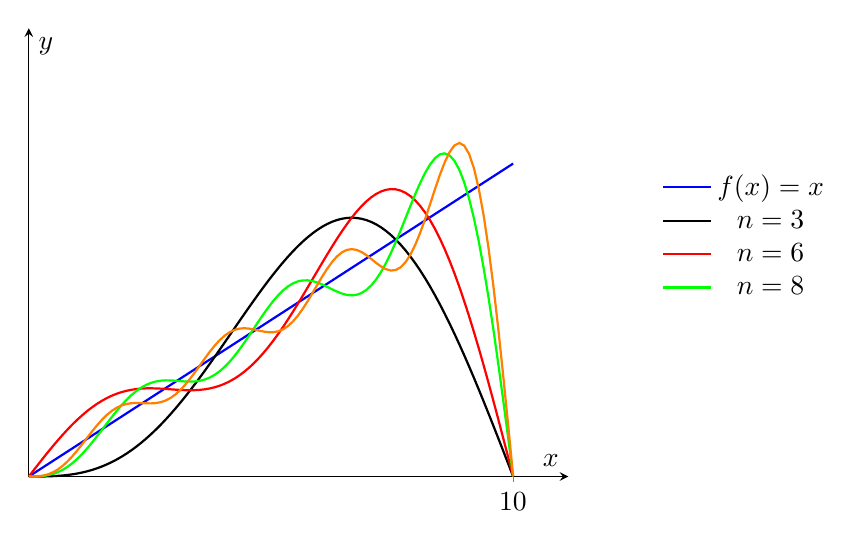
\begin{tikzpicture}
          \begin{axis}[
            domain=0:pi, samples=100,
            axis lines=middle,
            xlabel=\(x\), ylabel=\(y\),
            xmax=3.5, ymax=4.5, % Ajusta los valores según tus necesidades
            xtick={0, 3.14}, ytick=\empty,
            xticklabels={\(0\), \(10\)},
            enlargelimits=false,
            clip=false,
            legend style={at={(1.5,0.7)}, anchor=north east, draw=none}
          ]
            \addplot[blue, thick, domain=0:pi] {x};
            \addplot[black, thick, domain=0:pi] {2*sin(deg(x)) - sin(deg(2*x))};
            % Serie de Fourier en senos para n = 5
            \addplot[red, thick, domain=0:pi] {2*sin(deg(x)) - sin(deg(2*x))+ (2/3)*sin(deg(3*x))};
            % Serie de Fourier en senos para n = 7
            \addplot[green, thick, domain=0:pi] {2*sin(deg(x)) - sin(deg(2*x))+ (2/3)*sin(deg(3*x)) - (1/2)*sin(deg(4*x)) +  (2/5)*sin(deg(5*x)) - (2/6)*sin(deg(6*x))};
            % Serie de Fourier en senos para n = 10
            \addplot[orange, thick, domain=0:pi] {2*sin(deg(x)) - sin(deg(2*x))+ (2/3)*sin(deg(3*x)) - (1/2)*sin(deg(4*x)) +  (2/5)*sin(deg(5*x)) - (2/6)*sin(deg(6*x)) + (2/7)*sin(deg(7*x)) - (2/8)*sin(deg(8*x)) };

             \legend{\(f(x) = x\), \(n = 3\), \(n = 6\), \(n = 8\)};
          \end{axis}
        \end{tikzpicture}$$
    \end{sol}
    \item Sea $f$ una función periódica de periodo $2\pi$ e integrable Riemann. Comprobar que se puede expresar la suma $n$-ésima de Fourier como $$S_n(x) = \int_0^{2\pi} f(t) D_n(t - x) dt$$ para cierta función $D_n$.
    \begin{sol}
        Haciendo su desarollo en senos
        $$S_k(x)=\sum_{n=1}^k b_n \dfrac{\sin(kx)}{\sqrt{\pi}}=\int_0^{2\pi} f(t) D_k(t-x) dt$$
        y haciendo el desarrollo usual
        \begin{equation*}\begin{split} S_k(x)=&\left(\int_0^{2\pi} f(t) \dfrac{1}{\sqrt{2\pi}} dt\right)\dfrac{1}{\sqrt{2\pi}} + \mathlarger{\sum}_{n=1}^k \left(\int_0^{2\pi} f(t) \dfrac{\cos(nt)}{\sqrt{\pi}} dt \right)\dfrac{\cos(nx)}{\sqrt{\pi}} +\\
        &+\left(\int_0^{2\pi} f(t) \dfrac{\sin(nt)}{\sqrt{\pi}} dt \right)\dfrac{\sin(nx)}{\sqrt{\pi}}= \\
        &=\dfrac{1}{\pi} \left[ \int_0^{2\pi} f(t) \cdot \left(\dfrac{1}{2}+ \mathlarger{\sum}_{n=1}^k \cos(nt) \cos(nx) + \sin(nt) \sin (nx) \right)dt \right] = \\
        & = \int_0^{2\pi} f(t) \underbrace{\left[\dfrac{1}{2}+ \mathlarger{\sum}_{n=1}^k \dfrac{\cos(n(t-x))}{\pi} \right]}_{D_k(t-x)} dt
        \end{split}
        \end{equation*}
        donde a $D_k(t-x)$ se lo denomina \textbf{núcleo de Dirichlet}.
    \end{sol}
    \item Calcular la suma 
    $$\dfrac{1}{2} + e^{iu} + e^{2iu } + \cdots  + e^{niu}$$ 
    donde $i$ es la unidad imaginaria y $u \in \mathbb R$ (Indicación: es una suma geométrica). Tomando la parte real de la anterior suma, obtener una expresión para
     $$\dfrac{1}{2} +  \cos(u) + \cos(2u) + \cdots + \cos(nu)$$ 
    Aplicar lo anterior para demostrar que
    $$D_n(u) = \dfrac{1}{2\pi} \dfrac{\sin\left(\frac{2n+1}{2}u\right)}{\sin(\nicefrac{1}{2}u)}$$
    \begin{sol}
     La suma dada es una sucesión geométrica, de forma que 
     $$\dfrac{1}{2}+ e^{iu} + e^{2iu } + \cdots  + e^{niu} = \dfrac{1}{2}+ \sum_{i=1}^n (e^{iu})^n= \dfrac{1}{2}+ \dfrac{r-r^{n+1}}{1-r}=\dfrac{1}{2}+ e^{iu} \dfrac{1-e^{niu}}{1-e^{iu}} = \dfrac{1}{2}+ A$$
     Obsérvese que 
     $$e^{kiu}=\cos(kiu)+i\sin(kiu)=\mathfrak{R}\mathfrak{e}(e^{kiu})+i\: \mathfrak{I}\mathfrak{m}(e^{kiu}) \quad \forall k \in \mathbb N$$
     de forma que
     $$\mathfrak{R}\mathfrak{e}(A)=\dfrac{e^{iu}-1-e^{(k+1)iu}}{2(1-\cos(u))} + e^{kiu}=\dfrac{\cos(u)-1-\cos((k+1)u)+\cos(ku)}{2(1-\cos(u))}$$
     luego 
     \begin{equation*}
     \begin{split}\dfrac{1}{2}+\mathfrak{R}\mathfrak{e}(A)=&\dfrac{\cancel{\cos(u)}-\cancel{1}-\cos((k+1)u)+\cos(ku)+\cancel{1}-\cancel{\cos(u)}}{2(1-\cos(u))}=\\=&\dfrac{\cos(ku)-\cos((k+1)u)}{2(1-\cos(u))}=\\=& \dfrac{1}{\cancel{2}}\cdot \dfrac{-\cancel{2}\sin\left(\frac{2k+1}{2} \: u \right)\sin\left(-\frac{u}{2} \right)}{1-\cos(u)}=\\=&  \dfrac{\sin\left(\frac{2k+1}{2} \: u \right)\sin\left(\frac{u}{2} \right)}{2\sin^2\left(\frac{u}{2} \right)} =\\=&\dfrac{1}{2} \dfrac{\sin\left(\frac{2k+1}{2} \: u \right)}{\sin\left(\frac{u}{2} \right)}
     \end{split}\end{equation*}
    \end{sol}
    verificando así el enunciado.
\end{enumerate}